%% This is an example first chapter.  You should put chapter/appendix that you
%% write into a separate file, and add a line \include{yourfilename} to
%% main.tex, where `yourfilename.tex' is the name of the chapter/appendix file.
%% You can process specific files by typing their names in at the 
%% \files=
%% prompt when you run the file main.tex through LaTeX.
\chapter{Methodology}

The aim of machine learning methods is to train a model with a given data set in order to predict the output values corresponding to a new input. 

\section{Machine Learning}

According to Arthur Samuel, name father of machine learning, "Machine learning is the field of study that gives computers the ability to learn without being explicitly programmed". 
A rather more to the point but complicated definition offered by Tom Mitchell in 1998, quite new compared to Samuel\textquotesingle s in 1959, " A computer program is said to learn from experience E with respect to some task T and some performance measure P, if its performance on T, as measured by P, improves with experience E".

\subsection{Introduction}
Machine learning methods are mainly handled under two main categories: supervised and unsupervised learning as shown in Fig.~\ref{fig:machineLearningMethods}. 
In supervised learning, \textit{"right answer"} for each example in the data set is available to the user apriori. 
Whereas for unsupervised learning, the \textit{"right answer"} are not available. 
Although not as common as these methods, there are other machine learning algorithms serving specific purposes such as reinforcement learning and recommender systems. 
The common methodology in machine learning is that there are two phases, the learning and the prediction phases as in Fig.~\ref{fig:supervisedLearningBasics}. 

\begin{figure}
\begin{center}
\includegraphics[width=14cm]{figures/machineLearningMethods}    % The printed column width is 8.4 cm.
\caption{Common machine learning methodologies} 
\label{fig:machineLearningMethods}
\end{center}
\end{figure}

The first phase is comprised of learning from the available data to understand how the system behaves. 
In the second phase, the idea is to predict what will be the output of the system for a given input, depending on the knowledge about the system that you gained via learning phase. 

\begin{figure}
\begin{center}
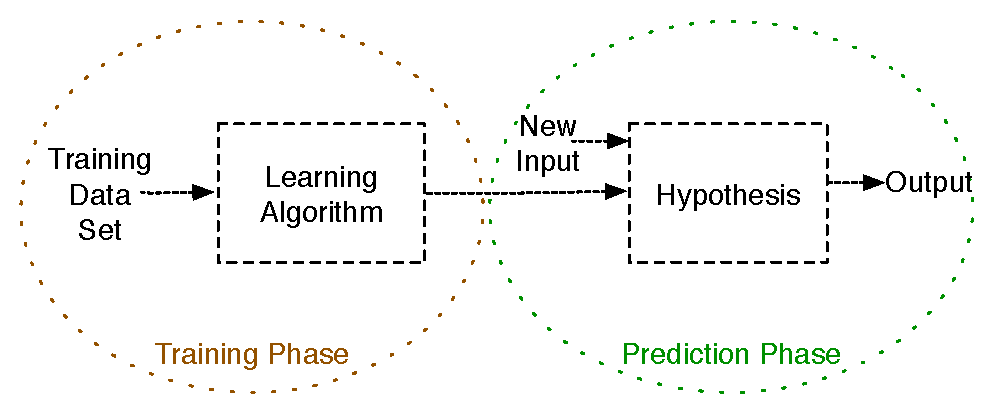
\includegraphics[width=14cm]{figures/supervisedLearningBasics}    % The printed column width is 8.4 cm.
% For the old picture 
% \includegraphics[width=12cm]{figures/machineLearningBasics}   
\caption{Supervised learning basics } 
\label{fig:supervisedLearningBasics}
\end{center}
\end{figure}
 
The most common types of supervised leaning is the regression and classification problems. 
Since these are both of supervised learning types, the \textit{"right answer"} (right values of the output $y$) for each example is assumed to be known. 

\subsection{Terminology}

Since being clear about the terminology is essential, a basic introduction to mostly used terms is given in this section.  
Table~\ref{arm:machineLearningTerminology} shows representations of commonly used variables in machine learning. 
Although representations could differ from one reference to the other, throughout this thesis, one coherent representation given in Table~\ref{arm:machineLearningTerminology} is followed. 

\begin{table}
\caption{Machine learning terminology}
\label{arm:machineLearningTerminology}
\begin{center}
\begin{tabular}{||l|l||}\hline
x & input variable or feature \\\hline
y & output variable or target variable \\\hline
\textbf{x} & input variable vector or feature vector \\\hline
\textbf{y} & output variable vector or target variable vector \\\hline
m & number of training examples \\\hline
n & number of features \\\hline
i & index of training examples \\\hline
j & index of features \\\hline
$\textbf{x}_j^{(i)}$ & $i^{th}$ training example for feature $j$ \\\hline
$\textbf{y}^{(i)}$ & $i^{th}$ training output  \\\hline
$\textbf{h}_{\bm{\theta}}(\textbf{x})$ &training output  \\\hline
$\textbf{J}({\bm{\theta}})$ &cost function  \\\hline

\end{tabular}
\end{center}
\end{table}

\begin{table}
\caption{Training set $(\textbf{x},\textbf{y})$ of housing prices - one-feature example}
\label{arm:exampHousingPrices}
\begin{center}
\begin{tabular}{ ||p{3cm}|p{3cm}|p{3cm}||}\hline
\textbf{training example index} $(i)$ & \textbf{Size in $feet^2$} ($\textbf{x}$) & \textbf{Price in $1000 \$ s$} ($\textbf{y}$) \\\hline
1 & 2104	   & 460 \\\hline
2 & 1416	   & 232 \\\hline
3 & 1534	   & 315 \\\hline
4 & 852	   & 178 \\\hline
$\vdots$ & $x^{(i)}$   & $y^{(i)}$ \\\hline
m & $x^{(m)}$   & $y^{(m)}$ \\\hline
\end{tabular}
\end{center}
\end{table}

Many of the machine learning tools have defaults settings and easy to be used by beginners. 
Although they would most probably not achieve optimized results which would be the case in the hands of an experienced user, a beginner can easily start using those tools by sending input and output vectors as arguments to the machine learning functions. 

The configurations of input and output vectors to feed the learning algorithms might change from one to other but still there is a common convention that would be compatible with many. 
In this representation, each instance is given in different rows of the input vector. 
An example of predicting housing prices (taken from Andrew Ng's machine learning course) is given to show the way to constitute the input and output matrix. 
Table~\ref{arm:exampHousingPrices} uses a supervised learning regression example to show input and output vector representations. 
The aim of the problem in this example is to predict price of houses for given surface area. 
For that, known examples of houses with surface area and corresponding price have been given. 
Since the aim of the problem is to predict the price of a house given the surface area, price of house is the output of the problem. 
And to predict the price, the available information that is known to effect the price of a house is the surface area of the house, making it the input variable. 
So, in Table~\ref{arm:exampHousingPrices} each row corresponds to a different house, second column (surface area of house) constitute the input vector and the last row (price in 1000s) corresponds to the output vector. 

In this problem, there is an assumption that the price of a house is only dependent on the surface area which would not hold in the real case. 
In real problems, it is more common that the output would depend not only one variable but more, or many. 
For that reason, the input vector in a realistic example would rather be an input matrix having different features in its columns as given in Table~\ref{arm:exampleMultiFeatures}. 
Here in this example, the output is still the price of house, but now the features which corresponds to each column of an input matrix (or sometimes called the feature matrix) are surface area, number of bedrooms, and can be enlarged until n features. 
It should be kept in mind the selection of features that would lead to a better prediction of the output is a challenging problem and usually requires experience on the system of interest. 

\begin{table}
\caption{Training set $(\textbf{x},\textbf{y})$ of housing prices - multi-feature example}
\label{arm:exampleMultiFeatures}
\begin{center}
\begin{tabular}{ ||p{2cm}|p{2cm}|p{2cm}|p{2cm}|p{2cm}|p{2cm}||}\hline
\textbf{training example index} $(i)$ & \textbf{Size in $feet^2$} ($\textbf{x}_1^{(i)}$) & \textbf{Number of bedrooms} ($\textbf{x}_2^{(i)}$) & \textbf{Feature j} ($\textbf{x}_j^{(i)}$) & \textbf{Feature n} ($\textbf{x}_n^{(i)}$) &\textbf{Price in $1000 \$ s$} ($\textbf{y}$) \\\hline
1 & 2104	& 5  & $\textbf{x}_j^{(1)}$ & $\textbf{x}_n^{(1)}$ & 460 \\\hline
2 & 1416 & 3 & $\textbf{x}_j^{(2)}$ & $\textbf{x}_n^{(2)}$ & 232 \\\hline
3 & 1534 & 3 & $\textbf{x}_j^{(3)}$ & $\textbf{x}_n^{(3)}$ & 315 \\\hline
4 & 852 & 2 & $\textbf{x}_j^{(4)}$ & $\textbf{x}_n^{(4)}$ & 178 \\\hline
$\vdots$ & $\textbf{x}_1^{(i)}$  & $\textbf{x}_2^{(i)}$  & $\textbf{x}_j^{(i)}$   & $\textbf{x}_n^{(i)}$ & $\textbf{y}^{(i)}$ \\\hline
m & $\textbf{x}_1^{(m)}$  & $\textbf{x}_2^{(m)}$  & $\textbf{x}_2j^{(m)}$   & $\textbf{x}_n^{(m)}$ & $\textbf{y}^{(m)}$ \\\hline
\end{tabular}
\end{center}
\end{table}


%\clearpage
%\newpage


\subsection{Steps towards the learning machine}

\subsubsection{Visualizing the data}

Having a preliminary glance at data might give the designer an idea about the ways to tackle the problem since it is the designer to select the features, the hypothesis, and the type of cost function. It is true that the algorithms are optimizing some parameters of the hypothesis and the cost function but still the structure itself is usually supplied by a human. 
Although there are tricks to select those in a better sense, machines still have a way to go towards Skynet.

% I AM HERE

Fig.~\ref{fig:housingPrices} shows the housing price depending on the surface area corresponding to the data given in Table~\ref{arm:exampHousingPrices}.
In this example, price of the houses are the output (target) variable given in y-axis and size (surface area in $feet^2$) is the feature (input) variable given in x-axis. 
Since output y is price which is a continuous value (thus not a label representing a class) this problem is called a regression problem. Plotting the data given shows that the problem could to be modeled by a linear hypothesis (a linear line to fit the data given). Then linear regression can be applied.

\begin{figure}
\begin{center}
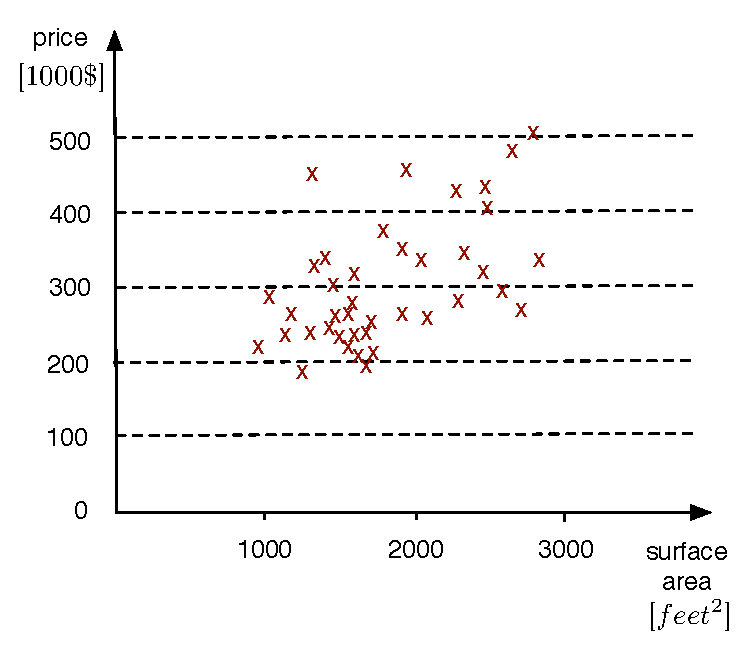
\includegraphics[width=11cm]{figures/linearRegressionExamp}    % The printed column width is 8.4 cm.
\caption{Linear regression example - Housing prices as a function of area of the house} 
\label{fig:housingPrices}
\end{center}
\end{figure}

\begin{figure}
\begin{center}
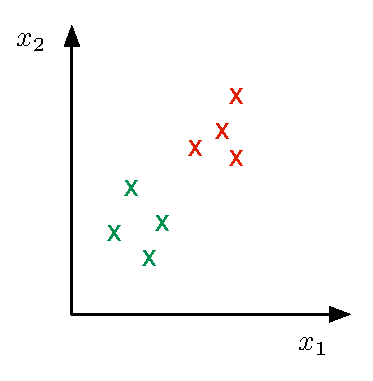
\includegraphics[width=5cm]{figures/classificationEx2}    % The printed column width is 8.4 cm.
\caption{Classification example} 
\label{fig:classificationEx2}
\end{center}
\end{figure}

Since an example for regression problem has been given, now a preliminary look at classification problem will be presented. 
Fig.~\ref{fig:classificationEx2} is a classification problem since the aim is to distinguish the class that a new input instance will belong to. 
Here the vertical dimension is not the output as in the previous example of linear regression but is another feature ($x_2$ in this example). 

And the information about the output is represented with the colors of the samples in the feature space.
Fig.~\ref{fig:classificationEx1} shows the output vs. inputs of a classification problem. 
This is just to show the difference between regression and classification problem figures. 
Usually in regression problems the y-axis represents the output. 
Here there is a direct analogy by representing a classification problem just as a regression problem, x-axis representing the input whereas y-axis representing the output. 
But usually in classification problems, value of y (which class it corresponds to) is represented with different colors as in Fig.~\ref{fig:classificationEx2} or with different signs such as O and X.

By just plotting the samples, in this example, it seems that logistic regression could yield satisfactory results since the data seems to be separated by a linear decision boundary. 

It is possible to choose the model structure that would represent the problem satisfactorily via visualizing the data set when the number of features are not large.
With an increasing number of feature set, determining the degree of the polynomial via visualizing data to represent the input output relationship could be more complicated. 
In that case, the user should refer to model selection techniques rather than the insights gained by data visualization. 


\begin{figure}
\begin{center}
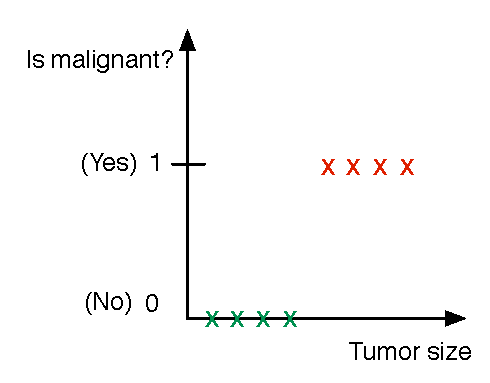
\includegraphics[width=7cm]{figures/classificationEx1}    % The printed column width is 8.4 cm.
\caption{Classification example} 
\label{fig:classificationEx1}
\end{center}
\end{figure}


In case the number of feature set is small but yet the visualization gives that the model for regression or classification problem can not be represented by a linear model (or linear decision boundary) feature mapping could be applied. 
Then linear regression or logistic regression (can only fit linear models unless features are mapped) could be applied to nonlinear systems with mapped features.  

\subsubsection{Feature Mapping}

This section applies to problems with smaller feature sets and to fit a nonlinear model with linear or logistic regression.
Depending on the results from visualizing data, it might be necessary to map the features since a straightforward implementation of linear / logistic regression will end up in linear model, linear decision boundary respectively. 
So for cases that the model or decision boundary being linear will not be enough to satisfactorily describe the training data, feature mapping should be applied.

The housing price problem can be revisited here to show how could feature mapping be done in that specific example.
The data given in Table~\ref{arm:exampHousingPrices} 

\begin{align}
\label{eqn:costFuncExamp1}
\begin{split}
h_{\theta}(x) & = \theta_0 + \theta_1 x_1 + \theta_2 x_2 + \theta_3 x_3
\\
& = \theta_0 + \theta_1 (size) + \theta_2 {(size)}^2 + \theta_3 {(size)}^3
\end{split}
\end{align}

where

\begin{align}
\label{eqn:featureMapping1}
\begin{split}
x_1 & = size
\\
x_2 & = size^2
\\
x_3 & = size^3
\end{split}
\end{align}

Below you can see a data set that will be used for logistic regression 
for the purpose of classification of a microchip assessment. 
It is seen from the plot that a linear decision boundary will 
not serve appropriately. So we might map our features as below

\begin{equation}{\label{eqn:featureMapping2}}
\bm{x_{mapped}}
=\,
\begin{bmatrix}
1 & x_1 & x_2 & x_1^2 & x_1x_2 & x_2^2 & x_1^3 \cdots & x_1x_2^5 & x_2^6 
\end{bmatrix}
\,^ T
\end{equation} 

\begin{figure}
\begin{center}
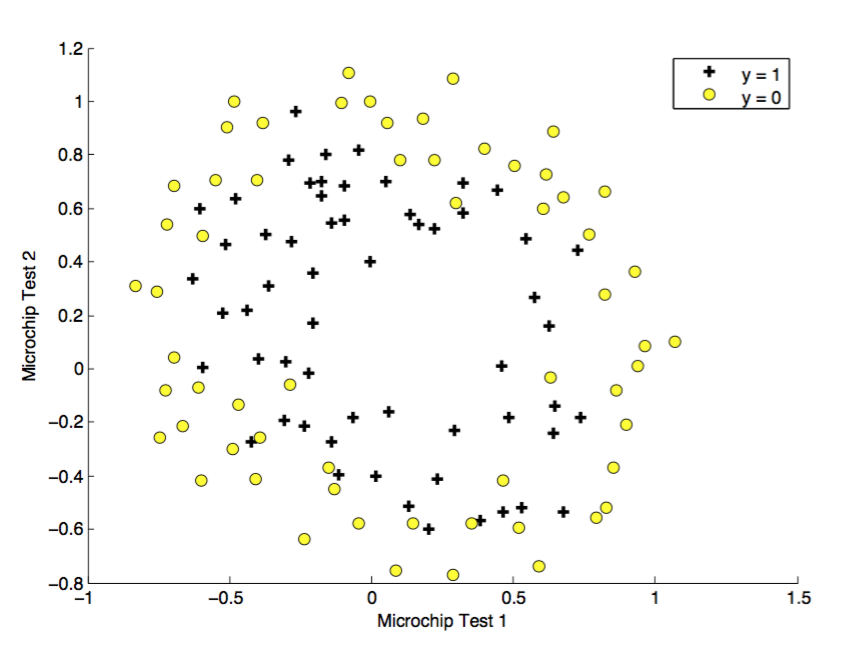
\includegraphics[width=13cm]{figures/classificationMicrochip}    % The printed column width is 8.4 cm.
\caption{Classification example} 
\label{fig:classificationEx3}
\end{center}
\end{figure}

To give an example of how many features you will inject 
into the problem, assume a binary classification problem 
with 100 features originally. Since the basic version of the 
logistic regression can fit a linear decision boundary only, 
let\textquotesingle s say that we will map the feature set 
such that only we take the quadratic terms, the new feature set becomes
 
\begin{equation}{\label{eqn:featureMapping3}}
\bm{x_{mapped}}
=\,
\begin{bmatrix}
x_1^2 & x_1x_2 & x_1x_3 & \cdots & x_1x_{100} & x_2^2 & x_2x_3 & \cdots & x_3^2 & x_3x_4  \cdots  
\end{bmatrix}
\,^ T
\end{equation} 

with a complexity $O(n^2) \sim \frac{n^2}{2}$

If you consider the 3rd order terms, the new feature set 
becomes

\begin{equation}{\label{eqn:featureMapping4}}
\bm{x_{mapped}}
=\,
\begin{bmatrix}
x_1^3 & x_1x_2x_3 & x_1^2x_2 & \cdots  & x_{11}x_{13}x_{17} & \cdots  
\end{bmatrix}
\,^ T
\end{equation} 

But keep in mind that with a higher dimensional feature vector, 
overfitting might become a problem. Which can be handled 
via regularization (Step 6). And also it could be computationally 
expensive as well.

To fit a model or decision boundary of a circular or elliptical 
shape, you might consider only the subset of features such that

\begin{equation}{\label{eqn:featureMappin54}}
\bm{x_{mapped}}
=\,
\begin{bmatrix}
x_1^2 & x_2^2 & x_3^2 & \cdots & x_N^2  
\end{bmatrix}
\,^ T
\end{equation} 

So the number of features will be less but it can not fit complex 
models or boundaries such as in Fig.~\ref{fig:complexBoundary}. 
You have to  consider more terms such as given in 
Equ.~\ref{eqn:featureMapping3} or you can use Neural Networks.
A scheme to help select the strategy for mapping is given in  Fig.~\ref{fig:ml_followChart}. 

\begin{figure}
\begin{center}
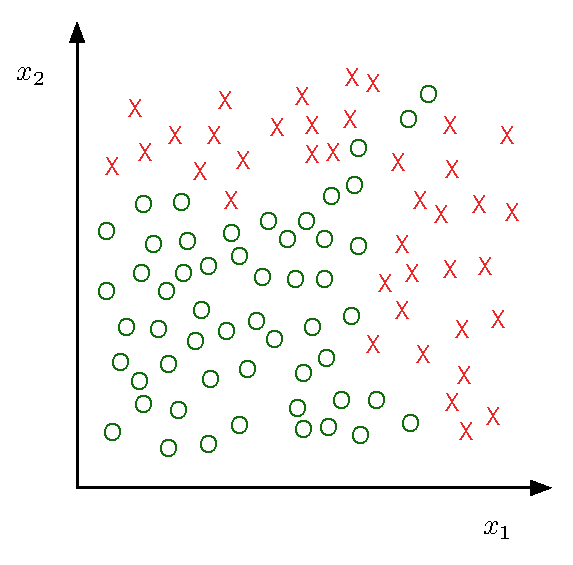
\includegraphics[width=6cm]{figures/complexDecisionBoundary}    % The printed column width is 8.4 cm.
\caption{Complex decision boundary} 
\label{fig:complexBoundary}
\end{center}
\end{figure}

\begin{figure}
\begin{center}
\includegraphics[width=14.7cm]{figures/ml_followChart}    % The printed column width is 8.4 cm.
\caption{Guide for feature mapping} 
\label{fig:ml_followChart}
\end{center}
\end{figure}

\subsubsection{Selecting Model Structure}

If you have more than one features, it might be difficult 
to have a sense of which model to choose. The idea 
behind selecting the model or realizing if your hypothesis 
is overfitting or not is to realize that when you fit some 
parameter by using some data, it might not be fair to 
judge if it is a good fit or not by using the same data set.   
Because in that case, the result could end up by modeling 
only that data well but not able to generalize to the new 
data which is our aim in the first place. So the idea is to 
have different subsets of data to train the model (calculating 
the model), to train the dimension of the model and to test if 
we trained them accurate enough to generalize to the new data set. 
The difference between calculating the test set error for 
overfitting (to distinguish if the model is over-fit or not) and 
calculating the test set error here for model structure 
selection is that we split the data set to 2 and 3 respectively. 
The difference in numbers is due to a common sense that 
when we fit a parameter, we should test it on a different data 
set to not to have a biased sense of error (the fitting check 
will give better results on the same data set it is trained on). 
In model structure selection problem we have an extra 
parameter we fit (unless it is not obvious that you fit that 
kind of an extra parameter.) This parameter is the model 
structure number (d). So when we select which model we 
choose we should calculate the error of our choice with a 
different data set. So we need 3 distinct data sets for that 
problem, to train parameters theta, select the model, and 
associate an error value with that choice. If we had two 
data set, and we calculate the test set error with the same 
data that we have used for selecting the model, than the 
error for selecting that model will be biased since it is the 
same data we used for selecting it. 

Fig.~\ref{fig:modelSelection}. 



\begin{landscape}
\begin{figure}
\begin{center}
%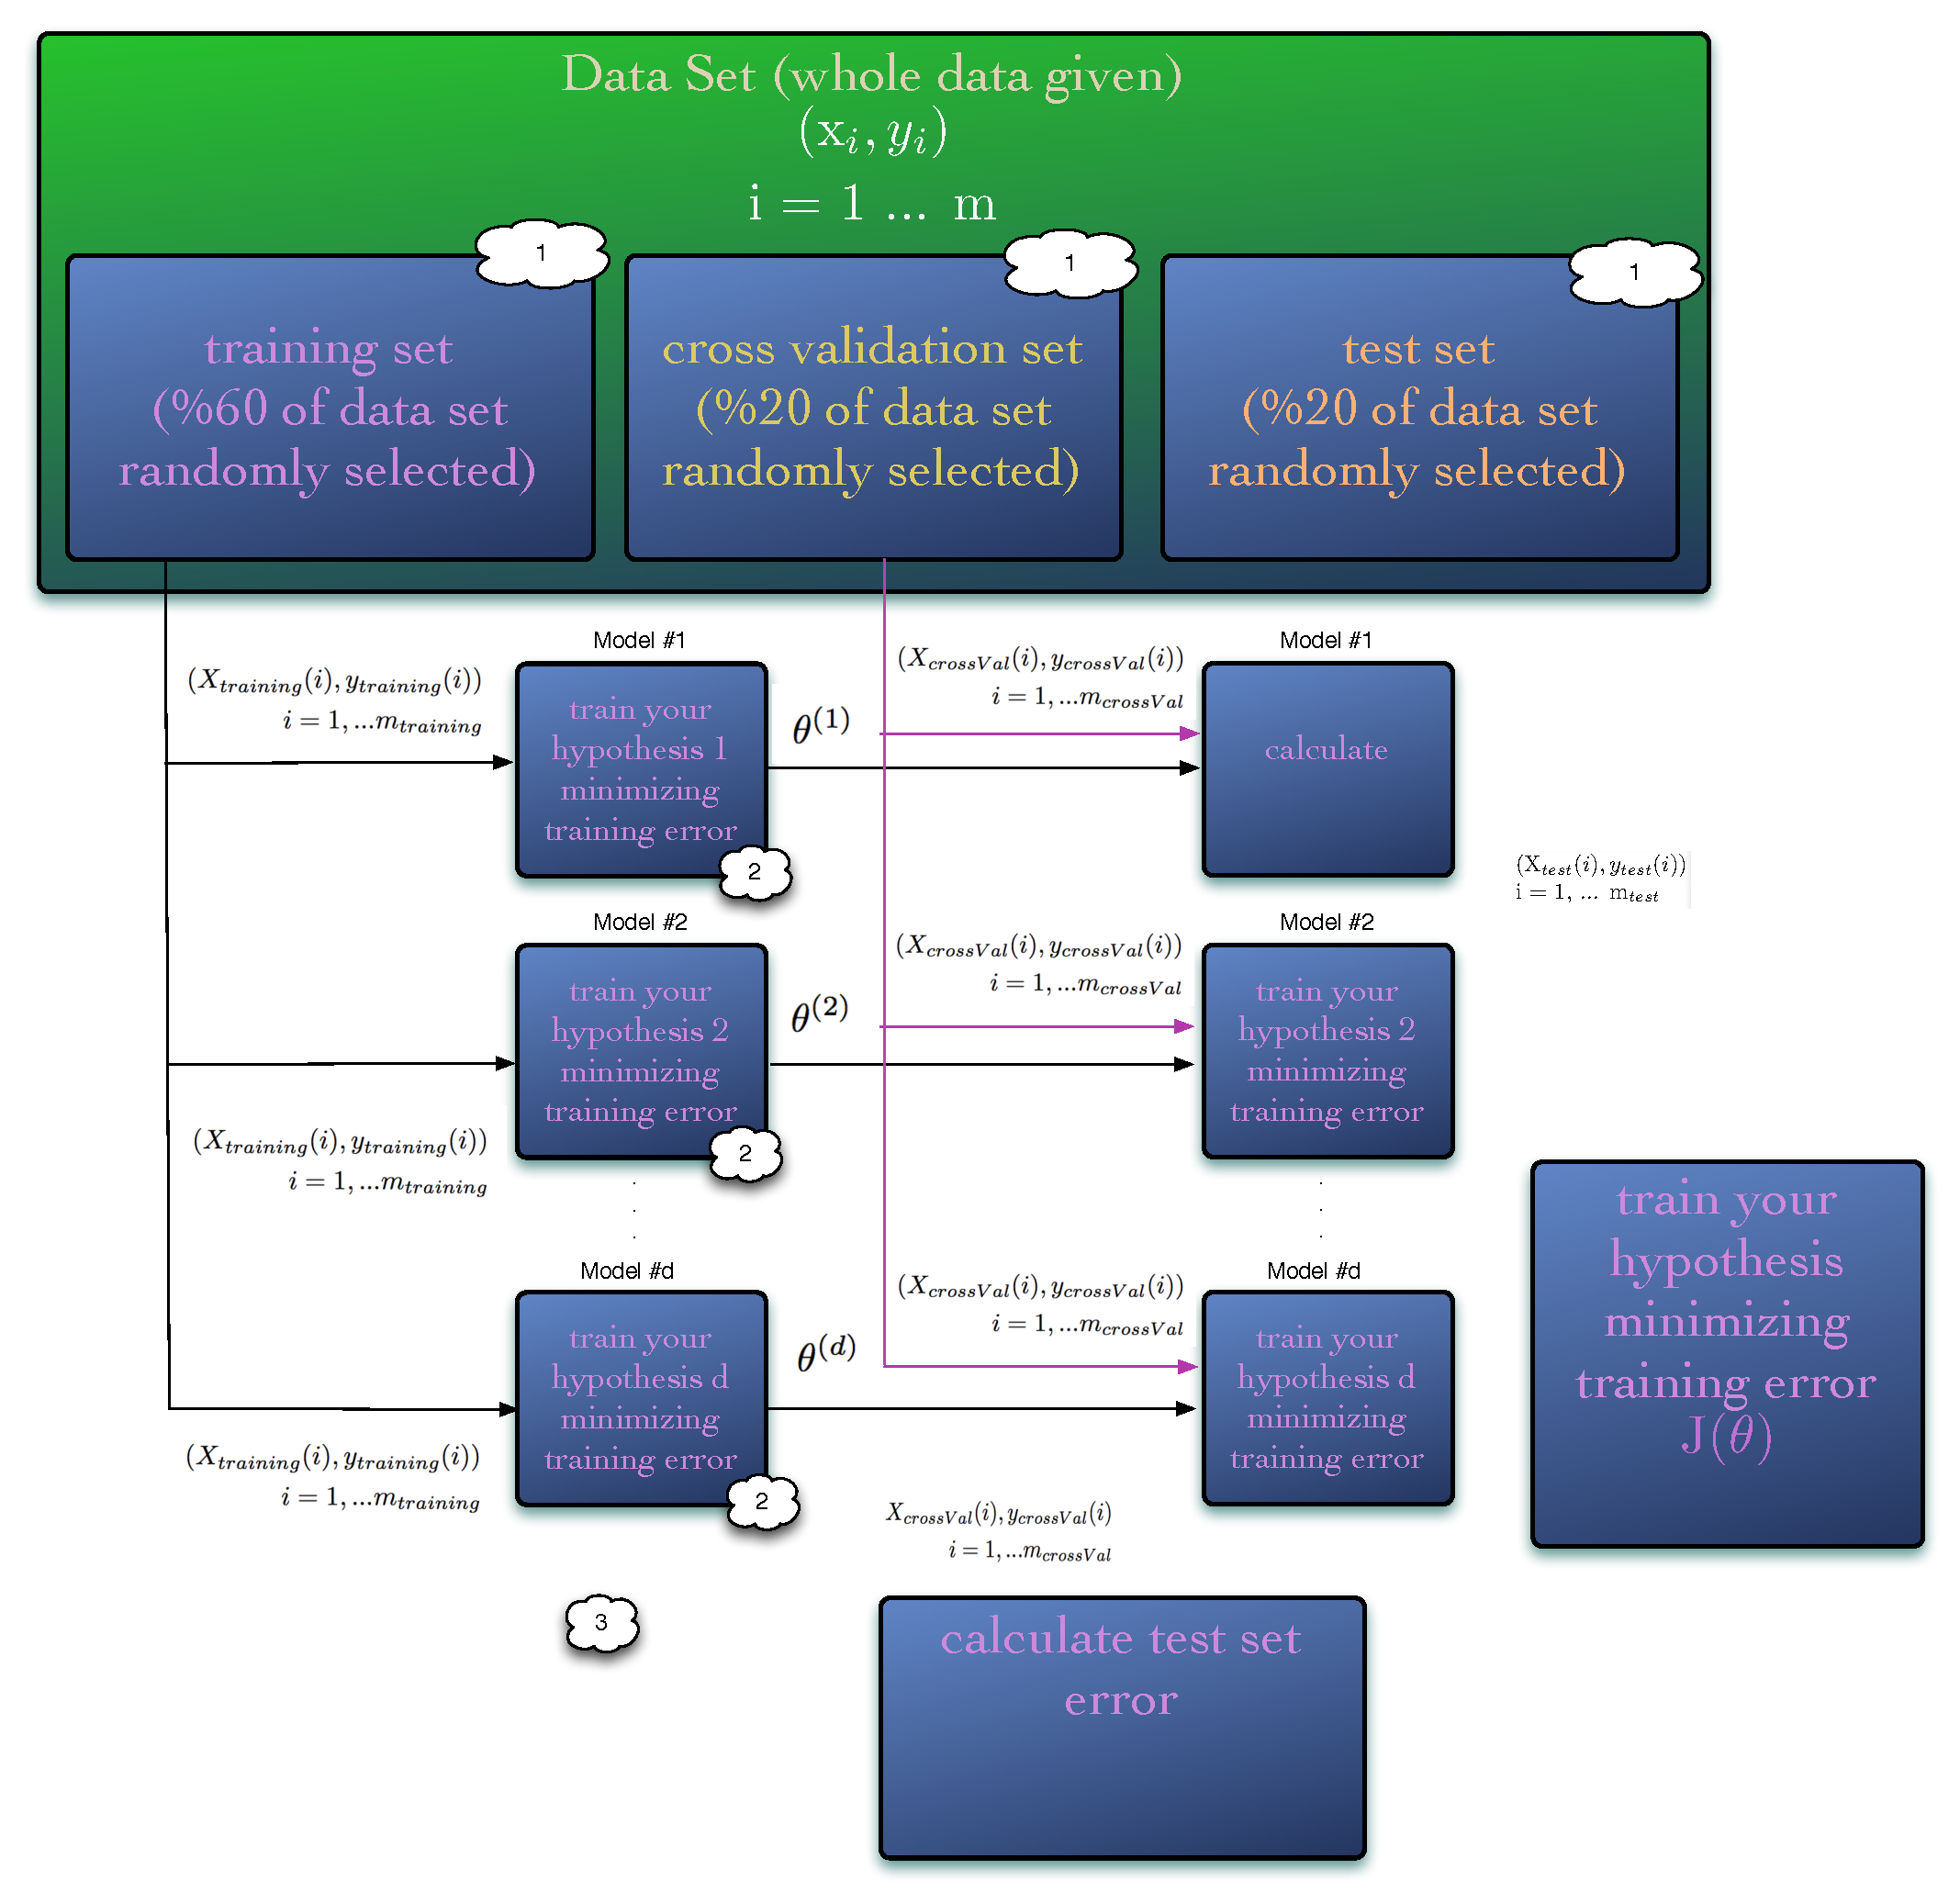
\includegraphics[width=16cm]{figures/modelSelection}    % The printed column width is 8.4 cm.
\includegraphics[width=23cm]{figures/modelSelectionNonVisualizableData}    % The printed column width is 8.4 cm.
\caption{Guide for feature mapping} 
\label{fig:modelSelection}
\end{center}
\end{figure}
\end{landscape}

Here the idea is to 

\begin{enumerate}
  \item Train the hypothesis for each model (d = 1,2,3 .. 10 in the 
example below is the degree of polynomial) by using the training set 
(\%60 of whole data, randomly selected) which will give you the 
parameters of the hypothesis for the selected model. So you 
will end up with x number of  parameter matrices, where x is 
the number of models you try (in this example x = 10).
  \item Then by using the cross validation data set (\%20 of whole 
data, randomly selected) calculate cross validation error for each 
model and select the one (d) with the smallest error.

\begin{equation}{\label{eqn:costFuncCrossVal}}
J_{cv}(\theta)
=\,
\frac{1}{2m_{cv}} \sum\limits_{i=1}^{m_{cv}} \Big(h_\theta(x_{cv}^{(i)}) - (y_{cv}^{(i)})\Big)^2  
\end{equation} 

  \item Then by using the cross validation data set (\%20 of whole 
data, randomly selected) calculate cross validation error for each 
model and select the one (d) with the smallest error.

\begin{equation}{\label{eqn:costFuncTest}}
J_{test}(\theta)
=\,
\frac{1}{2m_{test}} \sum\limits_{i=1}^{m_{test}} \Big(h_\theta(x_{test}^{(i)}) - (y_{test}^{(i)})\Big)^2  
\end{equation} 

\end{enumerate}


\begin{alignat*}{6}
\label{eqn:exampCostFunc}
d &= 1, \quad h_{\theta}(x) \ && = \theta_0 + \theta_1 x\ \ && \longrightarrow \theta^{(1)}\ \ && \quad \longrightarrow J_{cv}(\theta^{(1)})\
\\
d &= 2, \quad h_{\theta}(x) \ && = \theta_0 + \theta_1 x + \theta_2 x^2 \ \ && \longrightarrow \theta^{(2)}\ \ && \quad \longrightarrow J_{cv}(\theta^{(2)})\
\\
d &= 3, \quad h_{\theta}(x) \ && = \theta_0 + \theta_1 x + \theta_2 x^2 + \theta_3 x^3\ \ && \longrightarrow \theta^{(3)}\ \ && \quad \longrightarrow J_{cv}(\theta^{(3)})\
\\
& \ &&\ \vdots \ &&\ \ &&\ 
\\
d &= k, \quad h_{\theta}(x) \ && = \theta_0 + \theta_1 x_1 + \cdots+ \theta_k x^k\ \ && \longrightarrow \theta^{(k)}\ \ && \quad \longrightarrow J_{cv}(\theta^{(k)})\
\end{alignat*}

Select the d which makes $J_{cv}(\theta^{(k)})$ minimum and then 
estimate generalization error for the test set $J_{test}(\theta^{(4)})$.

\subsubsection{Scaling}

The next step is to normalize the features of the data to make the 
values of features change with the same order of magnitude. 
The reason is about the calculation of parameters of the hypothesis 
via an optimization algorithm and its convergence rate.  
Although there are different methods for normalization, a common one is to manage it

\begin{equation}{\label{eqn:scalingFeatures}}
\bar{x}_j = \frac{x_j - \mu_j}{s_j} 
\end{equation} 

where the mean and range is given as

\begin{align}
\label{eqn:meandAndRange}
\begin{split}
\mu_j & = \frac{\sum\limits_{i=1}^m {x_j^i} }{m}
\\
s_j & = max(x_j) - min(x_j)
\end{split}
\end{align}

An important point is to keep that values $\mu_j, s_j$ and may be standard 
deviation if it is used instead of range $s_j$. During prediction phase,
the data first should be scaled with these values attained from learning data.
If you have already added artificial feature  $x_0 = 1$ (step 4), 
do not apply scaling to the artificial feature.

\subsubsection{Add Artificial Feature}

This is for the purposes of generalizing the hypothesis for more features 
and the ability to write it in vectorized form. 

Such that a multiple feature 

\begin{equation}{\label{eqn:featureVector}}
\vec{\bm{x}}
=\,
\begin{bmatrix}
x_0\quad x_1 \quad  x_2 \quad \cdots \quad x_n 
\end{bmatrix}
\,^T
\end{equation} 

where $x_0 = 1$ with a parameter vector 

\begin{equation}{\label{eqn:parameterVector}}
\vec{\bm{\theta}}
=\,
\begin{bmatrix}
\theta_0\quad \theta_1 \quad  \theta_2 \quad \cdots \quad \theta_n 
\end{bmatrix}
\,^T
\end{equation} 

since the hypothesis for linear regression is 

\begin{equation}{\label{eqn:costFuncOneFeature}}
h_{\theta}(x) = \theta_0 + \theta_1 x_1
\end{equation} 

for one feature and 

\begin{equation}{\label{eqn:costFuncMltplFeature}}
h_{\theta}(x) = \theta_0 + \theta_1 x_1 + \theta_2 x_2 + \cdots+ \theta_n x_n
\end{equation}

for multiple features. The more common way to denote hypothesis in 
an compact generic form is 

\begin{equation}{\label{eqn:costFuncMltplFeature}}
h_{\theta}(x) = {\vec{\bm{\theta}}}^\intercal
\end{equation}

\begin{figure}
\begin{center}
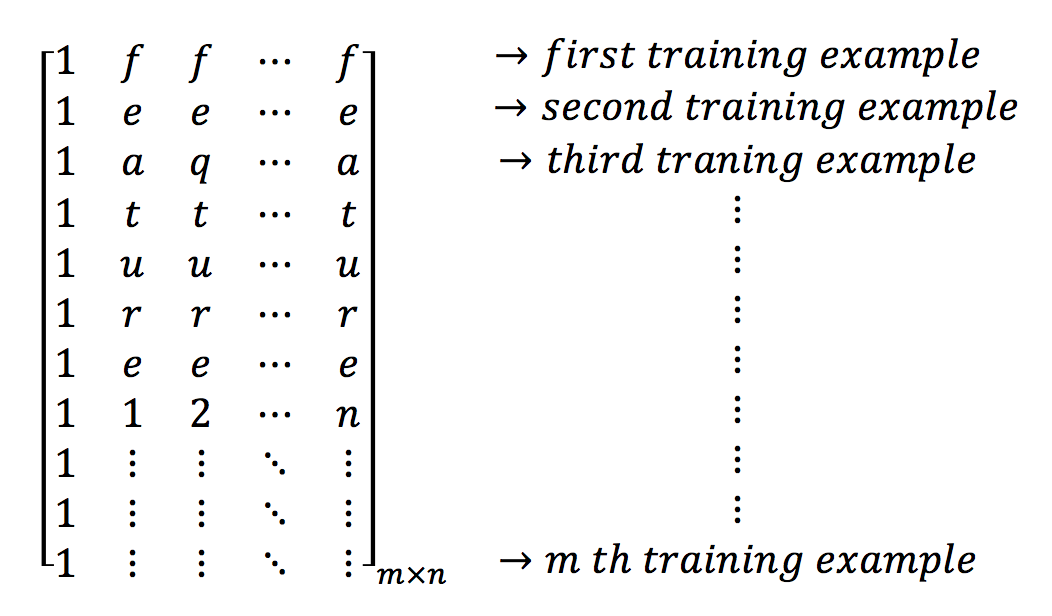
\includegraphics[width=9cm]{figures/addArtificialFeature}    % The printed column width is 8.4 cm.
\caption{Adding an artificial feature of 1s.} 
\label{fig:addArtificialFeature}
\end{center}
\end{figure}

Fig.~\ref{fig:addArtificialFeature}. 

\subsubsection{Selection of the Cost Function and Calculating the Gradient }

Cost function and the gradient are usually the inputs of the optimization 
algorithms by which you will calculate the optimized $\theta$ values 
to fit a model or a decision boundary by using the data set given to you. 
The selection of cost function is another issue but for standard applications 
there are widely used cost functions for each type of machine learning 
(e.g linear regression, logistic regression). 

Some examples of cost functions is given as an example below. 
Cost function for Linear Regression 

\begin{equation}{\label{eqn:costFuncLinearRegression}}
J(\theta)
=\,
\frac{1}{2m} \sum\limits_{i=1}^{m} \Big(h_\theta(x^{(i)}) - (y^{(i)})\Big)^2  
\end{equation} 

Cost function for Logistic Regression (Classification) - a subcase of two class e.g $y \in \{0,1\}$ . 

\begin{equation}{\label{eqn:costFuncLogisticRegression}}
J(\theta)
=\,
\frac{1}{m} \sum\limits_{i=1}^{m} \Big[-y^{(i)}log(h_\theta(x^{(i)})) - (1-(y^{(i)}))log(1-h_\theta(x^{(i)}))\Big]
\end{equation} 

\subsubsection{Modify the Cost Function by Adding Regularization Term}

Regularization is done to avoid overfitting which can be 
roughly explained that it is when you end up with a very complicated 
model or decision boundary, especially when you have nonlinear feature 
terms such as below;

\begin{equation}{\label{eqn:featureMapping2}}
\bm{x_{mapped}}
=\,
\begin{bmatrix}
1 & x_1 & x_2 & x_1^2 & x_1x_2 & x_2^2 & x_1^3 \cdots & x_1x_2^5 & x_2^6 
\end{bmatrix}
\,^ T
\end{equation} 

Overfitting might end up by fitting very well with the training set, 
but fail to generalize to the new data for the prediction phase. 
This means that the training set error is not a good predictor for 
how well the hypothesis would do on new examples.

\begin{figure}
\begin{center}
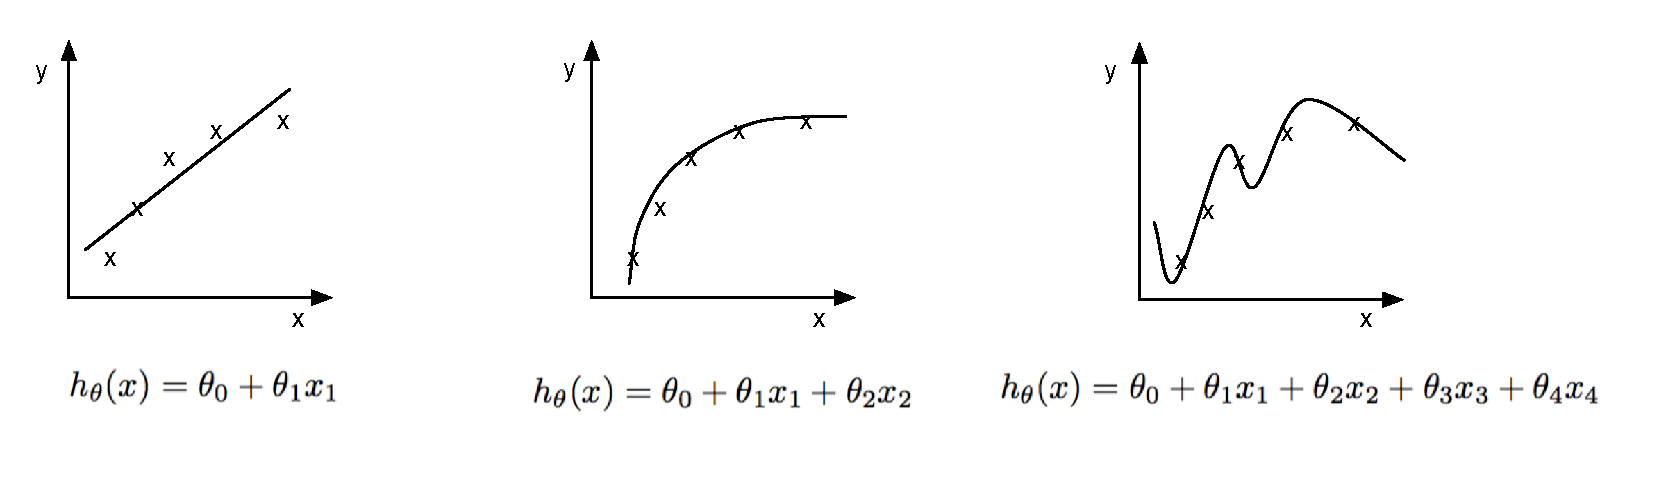
\includegraphics[width=16cm]{figures/underOverFit}    % The printed column width is 8.4 cm.
\caption{Guide for feature mapping} 
\label{fig:underOverFit}
\end{center}
\end{figure}

Fig.~\ref{fig:underOverFit} it is easy to realize that the hypothesis is under-fit, 
just right or over-fit since there is only one feature (plot and see). 
But for problems in which you have more features, it might not be 
that obvious or even not possible to plot and understand that the
 hypothesis is over-fit or not. For that cases the standard way to 
 evaluate the hypothesis
 
 \begin{enumerate}
 
  \item Split the data set you have to two portions 
  (\%30 for the test set - \%70 for the training set). 
  Note that if your data set is randomly ordered than you can 
  use the first \%70 for training and the rest for test, but if your 
  data is not randomly ordered (let\textquotesingle s say that we have data 
  set dependent on time), any kind of pattern in between 
  the data set, you should be randomly selecting this \%70 - \%30)
  
  \item Learn parameters theta from the new training set 
  (\% 70 of the whole data)

  \item Calculate the test set error by using test set 
  (\%30 of whole data) with the parameters you learned 
  by utilizing training set (\% 70 of the whole data).\\
  	For linear regression the test set error is the cost 
	function evaluated by the test set $(x_{test}(i), y_{test}(i))$ pairs 
	and the parameters trained by utilizing the new training set 
	(\% 70 of the whole data)
	
	\begin{equation}{\label{eqn:costFuncTest}}
	J_{test}(\theta)
	=\,
	\frac{1}{2m_{test}} \sum\limits_{i=1}^{m_{test}} \Big(h_\theta(x_{test}^{(i)}) - (y_{test}^{(i)})\Big)^2  
	\end{equation} 
	
	For logistic regression you either use the test set error
	
	\begin{equation}{\label{eqn:costFuncLogisticRegressionModified}}
	J_{test}(\theta)
	=\,
	-\frac{1}{m_{test}} \sum\limits_{i=1}^{m_{test}} \Big[y_{test}^{(i)}\,log(\ h_\theta(\ x_{test}^{(i)})) + (1-(y_{test}^{(i)}))\,log(\ h_\theta(\ x_{test}^{(i)}))\Big]
	\end{equation} 
	
	or the misclassification error (0/1 misclassification error)
	
	\begin{equation}{\label{eqn:errorMisclassificationError}}
	 test\ error
	=\,
	\frac{1}{m_{test}} \sum\limits_{i=1}^{m_{test}} \Big(err(\ h_\theta(\ x_{test}^{(i)}), (y_{test}^{(i)})\Big)  
	\end{equation} 

	\begin{equation}{\label{eqn:misclassificationError}}
	  err(h_{theta}(x),y)=\begin{cases}
               1 \qquad if\ h_{\theta}\geq0.5,\ y=0 \ or\ if \ h_{\theta} < 0.5, \ y=1\\
               0 \qquad otherwise\\
            \end{cases}
	\end{equation} 
		
\end{enumerate}

\begin{figure}
\begin{center}
\includegraphics[width=17cm]{figures/overfittingRealization}    % The printed column width is 8.4 cm.
\caption{Procedure to detect overfitting} 
\label{fig:overfittingRealization}
\end{center}
\end{figure}

To visualize the procedure, refer to  Fig.~\ref{fig:overfittingRealization}. 

\textbf{Regularization:}

You add a term to cost function to penalize parameters $\vec{\bm{\theta}}$
by being large (i.e to make $\vec{\bm{\theta}}$ as small as possible), 
but keep in mind that $\vec{\bm{\theta}}$ is not penalized (by convention).

\begin{equation}{\label{eqn:costFuncRegularized}}
J(\theta)
=\,
\frac{1}{2m} \bigg[ \sum\limits_{i=1}^{m} \Big(h_\theta(x^{(i)}) - (y^{(i)})\Big)^2 +\lambda \sum\limits_{j=1}^{n} \theta_j^2 \bigg] 
\end{equation} 

Here, the art is to find the appropriate value for lambda which serves 
like a weight between the usual part of the cost function and the second 
part, which penalize theta vector by being big. So it decreases the 
values of theta. But if this lambda is bigger than it supposed to be 
then you end up with 

\begin{equation}{\label{eqn:costFuncRegularizedTooMuch}}
h_\theta(x)
=\,
\theta_0 
\end{equation} 

since you penalized all terms except  (as we earlier said,  is not 
penalized by convention). Such that

\begin{equation}{\label{eqn:costFuncRegularizedTooMuchHow}}
h_\theta(x)
=\,
\theta_0 + \xcancel{\theta_1 x}  + \xcancel{\theta_2 x^2}  + \xcancel{\theta_2 x^3}  + \cdots + \xcancel{\theta_n x^n}
\end{equation} 

Thus you have an under-fit to the model such as

\subsubsection{Cost Function Minimization}

Here is the point to use the optimization algorithms to 
minimize cost function by changing the parameters $\vec{\bm{\theta}}$
(i.e not by changing x and y) which is represented mathematically as

\begin{equation}{\label{eqn:optimizationGoal}}
\underaccent{{\displaystyle \theta_0, \theta_1}}{minimize} \ J(\theta_0,\theta_1)
\end{equation} 

For that there are different optimization algorithms. One of them 
is the Gradient Descent.  Others are Conjugate Gradient, BFGS, L-BFGS. 
Most of them needs the cost function and its gradient to minimize the cost function. 
The selection of the optimization algorithm is another subject so for now you 
can select Gradient Descent.

\textbf{Gradient Descent:}

The gradient descent algorithm will be first given for one feature for simplicity 
for a linear regression model given as in Equ.~\ref{eqn:linearRegressionTwoFeaturesSummary}

\begin{align}
\label{eqn:linearRegressionTwoFeaturesSummary}
\begin{split}
h_{\theta}(x) & = \theta_0 + \theta_1 x_1 
\\
J(\theta_1,\theta_2)
 & =\,
\frac{1}{2m} \sum\limits_{i=1}^{m} \Big(h_\theta(x^{(i)}) - (y^{(i)})\Big)^2  
\end{split}
\end{align}

\begin{enumerate}
 \item The gradient descent for one feature is given below. 
 Beware that you have to simultaneously update the thetas, 
 meaning that you need to evaluate hypothesis in the summation just above with the previous theta values. So during one iteration, you should use the same theta values to substitute into $h_\theta(x)$, in order to calculate next values of $\theta_0, \theta_1$.
  \begin{algorithm}
   \caption{Gradient Descent for one feature only}
    \begin{algorithmic}[1]
      \Function{GradDesOneFeat}{$X, y, theta\_init, alpha, num\_iters$}       
      
      \Comment{Inputs: X - training inputs, y - training outputs, theta - parameters,\\ alpha - learning rate, num\_iters - 		number of iterations(termination condition)}

        \State $theta0 = theta(1))$  
        \State $theta1 = theta(2))$  
        \State $m = length(y)$ \Comment Number of training examples
%        \State Let $L[1 \ldots {n_1} + 1]$ and $R[1 \ldots {n_2} + 1]$ be new arrays

        \For{$j = 1$ to ${iter\_num}$} \Comment Do until satisfied
                \For{$j = 1$ to ${m}$}     \Comment Do for all training examples
                         \State initialize each grad to zero
           	 	\State $grad0 \leftarrow grad0 + (costFunc(x) - y)$
		         \State $grad1 \leftarrow grad1 + (costFunc(x) - y) * x$
                    \EndFor
                    \State $theta0 \leftarrow theta0 - alpha * grad0$
                    \State $theta1 \leftarrow theta1 - alpha * grad1$
        \EndFor
       \EndFunction

\end{algorithmic}
\end{algorithm}

 \begin{algorithm}
   \caption{Gradient Descent in a general sense}
    \begin{algorithmic}[1]
     \Function{GradDes}{$X, y, theta\_init, alpha, num\_iters$}    
           \State \textbf{Inputs:} X - training inputs, \\
           \qquad \qquad y - training outputs, \\
           \qquad \qquad theta\_init - initial guess for the optimized parameter theta,\\ 
           \qquad \qquad alpha - learning rate, \\
           \qquad \qquad num\_iters - number of iterations to find the optimized theta
           \State \textbf{Outputs:} theta - theta\_optimized/ theta vector that minimizes the cost function \\
           \qquad \qquad J - the values of the cost function calculated during the course of iterations
    \State repeat until convergence {
    \State $\theta_j \leftarrow \theta_j - \alpha \frac{\partial}{\partial \theta_j}J(\theta_0, \theta_1, \cdots)$
    	 \State For correct implementation, update simultaneously e.g
	 \State 	\qquad  $temp0 = \theta_0 - \alpha \frac{\partial}{\partial \theta_0}J(\theta_0, \theta_1, \cdots)$
	 \State 	\qquad  $temp1 = \theta_1 - \alpha \frac{\partial}{\partial \theta_1}J(\theta_0, \theta_1, \cdots)$
          \State 	\qquad  \qquad $\vdots$
          \State 	\qquad  $\theta_0 = temp0$
	 \State 	\qquad  $\theta_1 = temp1$
	 \State 	\qquad  \qquad $\vdots$
		 }
       \EndFunction
\end{algorithmic}
\end{algorithm}

 \item Choosing initial value of $\theta$ ($theta\_init$)
 
 A conventional approach is to assign $theta_init = 0$
A point to know is that for different initial values your 
 theta might converge to a different value  (local minima 
 but not the global one) as in Fig.~\ref{fig:localOrGlobalMinimaGD}. 
 But for linear regression it is shown 
 that the cost function that we have selected in the notes 
 above is convex, meaning that it has no local minima. 
 It has only one global minima. 

An example of different initial conditions will converge 
 to different solutions (slightly different choice of initial 
 theta might make you converge to the local minima, 
 which gives you $J(\bm{\theta})$ values smaller than some 
 parts but does not give you the smallest value of $J(\bm{\theta})$.

\begin{figure}
\begin{center}
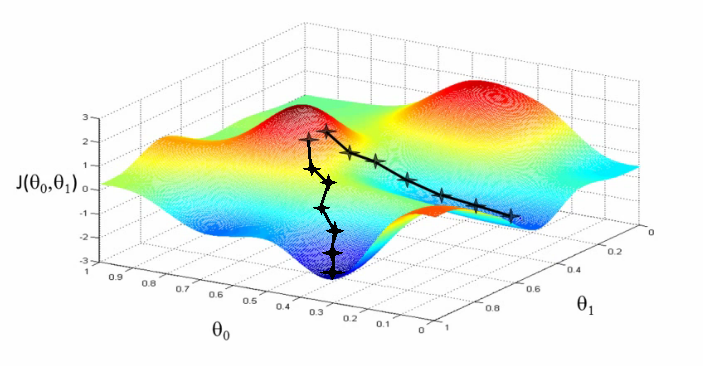
\includegraphics[width=11cm]{figures/localOrGlobalMinimaGD}    % The printed column width is 8.4 cm.
\caption{Gradient descent convergence dependance on $theta_init$. Two different but close choice of $theta_init$ might converge to local or global minima } 
\label{fig:localOrGlobalMinimaGD}
\end{center}
\end{figure}

 \item Choosing learning rate, $\alpha$ ($alpha$)
 
 Alpha, learning rate gives the gradient descent its step size, 
 so a bigger value means a faster convergence. But keep 
 in mind for a big alpha, your solution might not converge 
 or even diverge. And too small value might end up the 
 optimization to converge very slowly.
So you can try in order these values of $alpha = 0.001, 0.01, 0.1, 0.003, 0.03, 0.3$
 
\item Choosing number of iterations ($num\_iter$)
  
You might start with $num\_iter = 1000$  and then by visualizing 
the cost function check if the cost function converged to a steady 
value or not. If it has not yet converged but decreasing, 
try a bigger value for $num\_iter$
\end{enumerate}

\subsubsection{Visualizing the cost function}

Check converge by visualizing the cost function 
as a function of iterations of the optimization algorithm. 
Normally you expect this plot to be decreasing, 
never increase, converging to a steady value at 
the end of the optimization algorithm.

\begin{figure}
\begin{center}
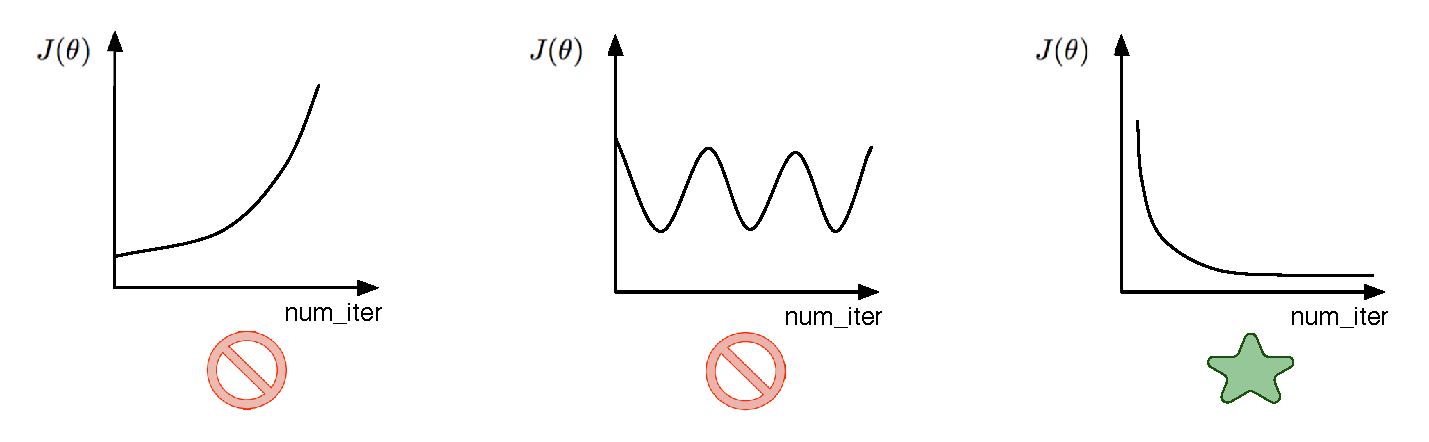
\includegraphics[width=15cm]{figures/visualizeCostFunc}    % The printed column width is 8.4 cm.
\caption{Evolution of $J(\theta)$ with respect to number of iterations. Left two figures showing that the optimization problem is not converging. The figure in the far right is the $J(\theta)$ evolution expected} 
\label{fig:visualizeCostFunc}
\end{center}
\end{figure}


To be able to observe how the cost function 
$J(\theta)$ during the iterative process of optimization, 
you should save the cost function values at each iteration.
Two examples of a bad optimization implementation can be seen in
Fig.~\ref{fig:visualizeCostFunc}. 

Not a good sign! Decrease alpha(learning rate)
What you expect is something like this Fig.~\ref{fig:visualizeCostFunc}. 


 WRITE SOME HERE Fig.~\ref{fig:debuggingHypothesis}
\begin{landscape}
\begin{figure}
\begin{center}
%\includegraphics[width=20cm,angle=90,origin=c]{figures/debuggingHypothesis}    % The printed column width is 8.4 cm.
\includegraphics[width=19cm]{figures/debuggingHypothesis}    % The printed column width is 8.4 cm.
\caption{Diagnosis the problem of machine learning by comparing the cost function for the training and cross-validation data sets} 
\label{fig:debuggingHypothesis}
\end{center}
\end{figure}
\end{landscape}

\subsubsection{Visualizing the model/classifier (decision boundary) with respect to training data}

Overfitting can be roughly explained that it is when you 
end up with a very complicated model or decision boundary. 
This ends up by fitting very well with the training set, but fail to 
generalize to the new data for the prediction phase. 
If overfitting occurs apply regularization meaning; Go step 6.

\subsubsection{Prediction}

For a new set of input data, now you will predict the outcome thanks to the model/classifier you trained. Now you should first normalize the new data $X_new$ by using the same mean and standard deviation values we had previously calculated from the training set. And then evaluate h(theta) by the optimized theta and regularized new data set $X\_new\_regul$. 

\section{Support Vector Machines}

\subsection{Introduction}

Let $ E = \Big\{ \big( \vec{\bm{x}}_1, y_1 \big),\big( \vec{\bm{x}}_2, y_2, 
		\cdots, \big( \vec{\bm{x}}_m, y_m \big) \big) \Big\}$, 
		where $\vec{\bm{x}}_i \in {\rm I\!R}^n$ and $y_i \in \big\{0, 1\big\}$ 
		be a training example set. Assuming the training data linearly separable, 
		

SVM is a relatively new approach for classification offering better generalization property thanks to its foundations on the structural risk minimization principle \cite{gunn1998support,yin2014study} while other classifiers usually only minimizes the empirical risk. This advances the capacity of generalization even with a small number of instances by reducing the risk of overfitting for a nicely tuned parameters setting. It can be applied to nonlinear systems and problems offering a vast number of features. Furthermore, taking advantage of convex optimization problems in the solution of SVM models, another attractive reason to use SVM rises as avoidance of global minimas, while Neural Networks is inherently prone to local minimas.

The idea behind SVM is to find an optimal hyperplane that will linearly separate the classes. This is achieved with the introduction of maximum margin concept which is the distance in between the boundaries when they are extended until hitting the first data point as in Fig.~\ref{fig:svmHyperplane}. The points closest to the hyperplane (decision boundary) are called the support vectors and are the representatives of the data sets to be used for the decision process. This helps to decrease the data to handle abruptly, enhancing the ability to cope with the curse of dimensionality and reducing the computational complexity.

SVM has other tricks to deal with not linearly separable problems such as using kernels to map data into higher dimensional feature spaces where they can be separated with a linear hyperplane.

\begin{figure}
\begin{center}
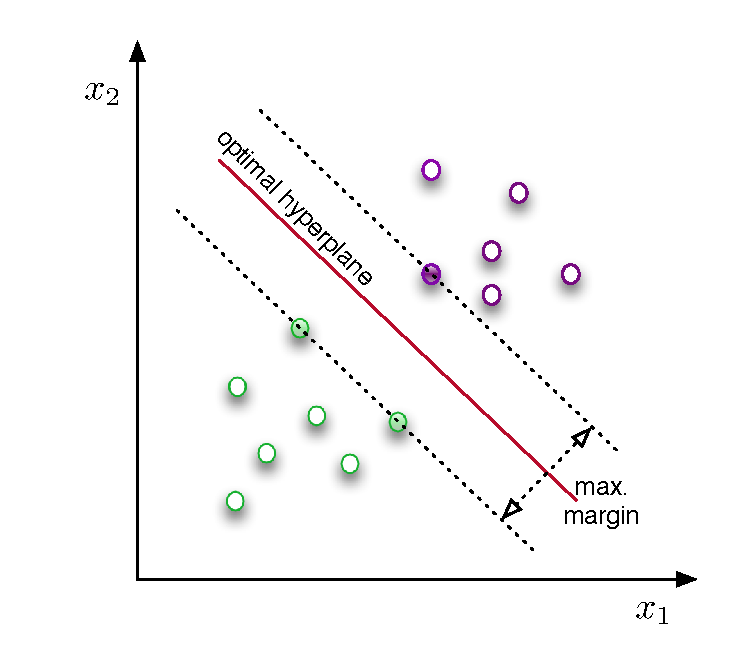
\includegraphics[width=9cm]{figures/svmHyperplane}    % The printed column width is 8.4 cm.
\caption{SVM working principle} 
\label{fig:svmHyperplane}
\end{center}
\end{figure}

A binary classifier is used in this work to classify two classes, faulty and nominal. The fault considered in this study is one of the control surface stuck at $0^{\circ}$. SVM being a supervised classification algorithm has two main phases as shown in Fig.~\ref{fig:supervisedLearning}. In the training phase, the model is learned as a fit to the labeled data that is fed to the SVM algorithm. This phase is usually followed with a tuning phase where some of the parameters of SVM is changed and results are compared to have the best fit via cross validation to avoid overfitting. The last phase is the prediction, where for a new instance the classifier predicts if it corresponds to a faulty or nominal condition.

Training data is comprised of labeled data where the label can belong to one of two possible cases. This data set is saved in $\bm{X} \in {\rm I\!R^{m \times n}}  $ where $m,n$ correspond to number of instances and features respectively. The label information corresponding to the measurement instances is also fed to the SVM algorithm during the training phase as output vector $\bm{y} \in \{-1,1\}$. The aim of SVM is to find an optimal hyperplane maximizing the margin by solving the optimization problem for non-linearly separable datasets

\begin{align}
min_{\gamma,\omega,b} \quad & \frac{1}{2} \norm{\omega}^2 + C \sum\limits_{i = 1}^m \xi_i \\
s.t. \quad & y^{i}(\omega^T x^(i) + b) \geq 1 - \xi_i, \ i = 1, \cdots, m\\
 & \xi_i \geq 0, \ i = 1, \cdots, m
% hic bir sey yazmazsan esitlikleri alt alta hizaliyor canim benim&=alo \\
% $ tek dolar arasi $ inline denklem
% $$ cift dolar arasi $$ satir atlayarak ortada denklem
\end{align}

To avoiding overfitting, which is the main problem of parametric discrimination approaches such as neural networks, parameter $C$ is tuned to result in the optimal fit for the cross validation set. The data set available is first divided to two portions with a percentage of \%20, \%80 where the bigger chunk is the training set and the remaining is the test set. Further, the training set is divided as cross-validation and training sets. The idea to split data is to avoid overfitting. Overfitting means that the models trained being very accurate fit for the data they are trained to but fail to generalize with new inputs resulting in bad prediction performance for the new data. To assess the performance of the classifier trained with the training data is tuned to give a better performance with the cross validation data. And then the final ability of the classifier is tested on the test set. This parameter also tuned for the outliers to generalize the distribution of the data rather than resulting in fine fits for each individual data in the training set. 
With a satisfactory result of the training \& tuning is followed by the prediction where the classifier predicts if the new measurement data belongs to the faulty or nominal class. The output of the SVM classification is not the probability that the new measurement belongs to one class as is in the traditional classification problems, but directly the class information it belongs to. For investigating the performance of the classifier on the test set, a method \cite{platt1999probabilistic} is used to calculate the posterior probabilities giving the probability that the new measurements belongs to faulty mode. Results shows as in  Fig.~\ref{fig:post_prob} that proper tuning achieves very accurate and instant detection for the drone fault.
 
\subsection{Application}

A binary classifier is used in this work to classify two classes, faulty and nominal. 
The faults considered in this study is the loss of effectiveness of the control surfaces and and the control surface stuck. 
Last section explains how the faulty data generated in flight and then labeled on the ground to be fed to the classifier. 
In this section, the classification of the faults will be explained in detail. 

SVM being a supervised classification algorithm has two main phases as shown in Fig.~\ref{fig:supervisedLearning}: training and prediction. 
The labeled data set is first divided to two portions with a percentage of \%20, \%80 where the bigger chunk is the training set and the remaining is the test set. 
Further, the training set is divided as cross-validation and training sets. The idea to split data is to avoid overfitting. 
Overfitting means that the models trained being very accurate fit for the data they are trained to but fail to generalize with new inputs resulting in bad prediction performance for the new data. 

\subsubsection{Training of the classifier}
In the training phase, the model is learned as a fit to the labeled data that is also an input to the SVM algorithm. 
Training data is comprised of labeled data where the label can belong to one of two possible cases. 
This data set is saved in $\bm{X} \in {\rm I\!R^{m \times n}}  $ where $m,n$ correspond to number of instances and number of features respectively. 
The label information corresponding to the measurement instances is also fed to the SVM algorithm during the training phase as output vector $\bm{y} \in \{-1,1\}$. 

The next step is to normalize the features of the data to make the values of features change with the same order of magnitude. 
The reason is due to its benefits to the calculation of parameters of the hypothesis via an optimization algorithm and its convergence rate.  
An important point is to keep that values $\mu_j, s_j$ and may be standard deviation if it is used instead of range $s_j$. 
During prediction phase, the data first should be scaled with these values attained from learning data.
If in the hypothesis artificial feature  $x_0 = 1$ is added to the features, do not apply scaling to the artificial feature, but this does not apply to SVM classification.

The aim of SVM is to find an optimal hyperplane maximizing the margin by solving the optimization problem for non-linearly separable datasets. 
SVM implements the idea of having a confidence in the prediction by using the concept of separating data with large margin. 
Some other classification methods, such as logistic regression, outputs the probability of a new instance's class, giving the confidence of the prediction as output inherently. 
On the other hand, SVM does only output if the new instance belongs to a class not necessarily pointing the confidence on this decision. 
Rather than including this confidence information as an output in terms of probabilities, this information is introduced with the functional and geometric margins. 
These definitions also serve for mathematically convenience, so that the optimization problem can be represented as a convex optimization problem.
Furthermore, introducing the Lagrange duality to obtain the dual form of the optimization problem, use of kernels, to work efficiently in higher dimensional spaces, is eased. 
The dual form also allows to utilize efficient optimization solvers such as Sequential Minimal Optimization (SMO)  \cite{platt1998sequential} which is the solver used in this work as well. Conventionally, training phase of SVM requires to solve a large quadratic programming (QP) problem. Especially for large training set, computational heaviness of this phase might limit the applicability of SVM to specific problems sets. To overcome this constraint, SMO breaks the QP problem into a series of smaller QP problems which can be solved analytically. Default settings for SVM binary classification, included in Matlab Statistics and Machine Learning Toolbox, utilizes SMO for optimization if outlier fractions has not been specified during the function call. 

%Tolerance for the gradient difference between upper and lower violators obtained by Sequential Minimal Optimization (SMO) or Iterative Single Data Algorithm (ISDA), specified as the comma-separated pair consisting of 'DeltaGradientTolerance' and a nonnegative scalar.
% The default values are: 1e-3 if the solver is SMO (for example, you set 'Solver','SMO')

Kernels are at the core of efficient SVM classifiers. A kernel, in general is defined as

\begin{equation}
K (x,z) = {\phi(x)}^T \phi(z)
\end{equation}

where $\phi$ represents the feature mapping. 
Default settings of Matlab's binary SVM classifier fits a linear model, which results in a linear decision boundary. 
If the system of interest requires a more complicated decision boundary to effectively classify the training data, mapping the original features might be necessary. 
Usually the original features of the systems are named as attributes while the mapped set are called the features. 
In other words, $\phi$ maps the attributes to the features. Kernels offer various elegant properties such as computational efficiency. 
Cleverly selected, SVM classifiers can learn in high dimensional spaces represented by $\phi$ without the need to explicitly find or represent $\phi$, but instead calculating $K(x,z)$, which might be computationally more efficient. 
In this study, Gaussian Kernel, which corresponds to an infinite dimensional feature mapping, is utilized to map the attributes.

\begin{equation}
K (x,z) = exp \bigg(-\frac{\Vert x - z \Vert ^ 2}{2 \sigma^2} \bigg)
\end{equation}

\subsubsection{Tuning of the classifier}
% HIGH VARIANCE = OVERFIT =   LARGE C = SMALL sigma^2
% HIGH BIAS = UNDERFIT = SMALL C =  LARGE sigma^2
% sigma^2 LARGE = HIGH BIAS 

Training phase is usually followed by a tuning phase where some of the parameters of SVM are tuned and results are compared in order to have the best fit via cross validation set. This is the phase where the parameters of the classifier are fixed to be used in the last phase, prediction.

\begin{figure}
\begin{center}
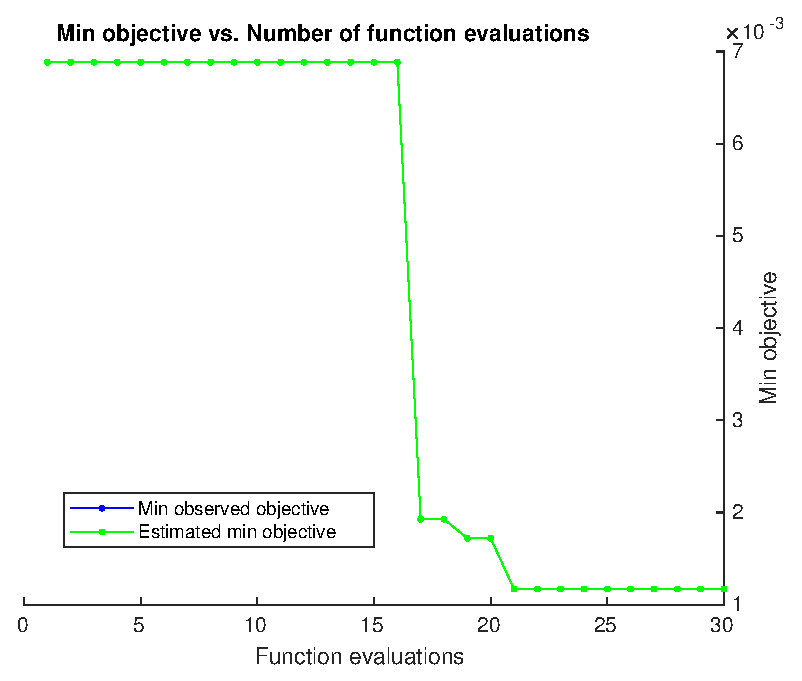
\includegraphics[width=0.7\textwidth]{figures/objectiveFuncEval}    % The printed column width is 8.4 cm.
\caption{Convergence of minimum objective function} 
\label{fig:objectiveFuncEval}
\end{center}
\end{figure}

\begin{figure}
\begin{center}
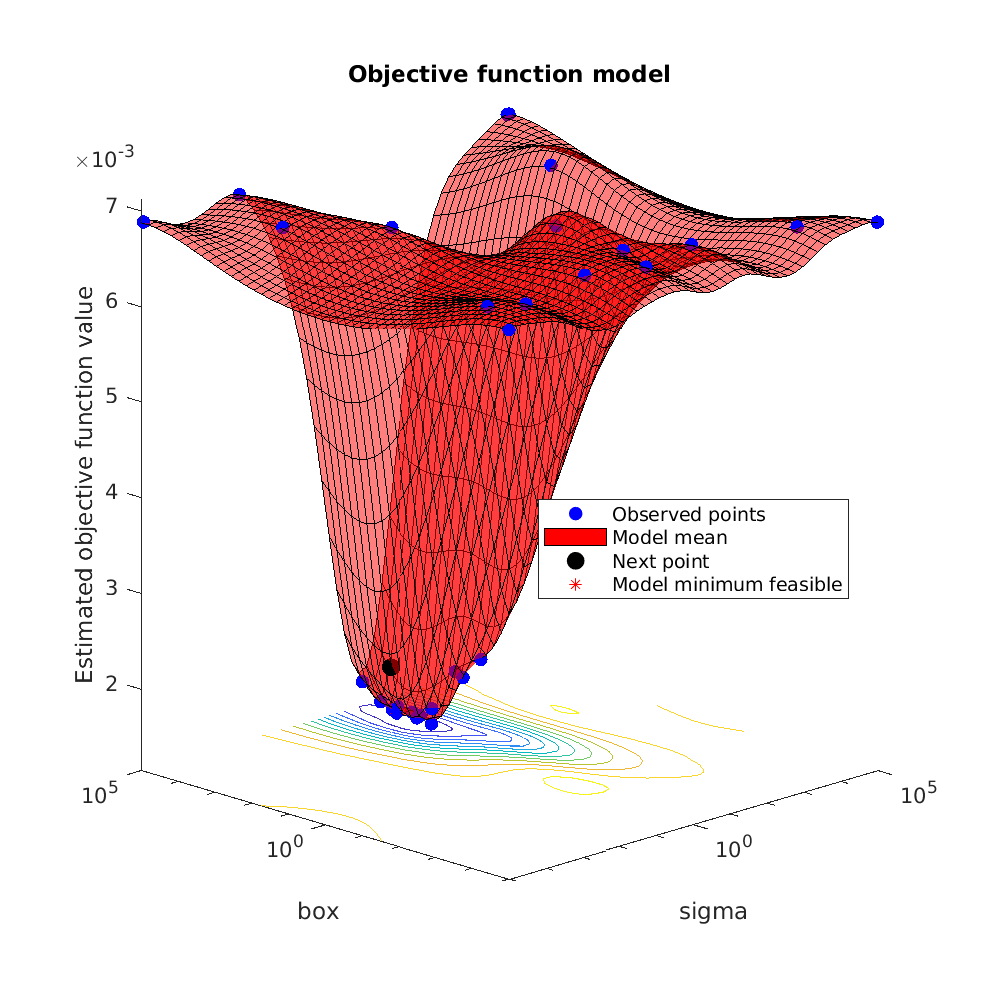
\includegraphics[width=0.7\textwidth]{figures/objFuncModel}    % The printed column width is 8.4 cm.
\caption{Objective function values for different box parameter and sigma values} 
\label{fig:objFuncModel}
\end{center}
\end{figure}

To avoiding overfitting, which is the main problem of parametric discrimination approaches such as neural networks, $C$ (box constraint) and the kernel scale (sigma), are tuned.
The classifier is trained with the training set and tuned via cross validation set, and then the selected classifier is evaluated with the test set. Cross-validation set selection of Matlab utilizes a random selection over the data set. 
To compare different methodologies for tuning and also the untuned classifiers, the script has been revised to generate random values from the same seed value to be consistent in comparisons.
Box constraint (C) and kernel scale (sigma) are tuned considering the presence of the outliers to generalize the distribution of the data rather than resulting in fine fits for each individual data in the training set. 

\begin{figure}
\begin{center}
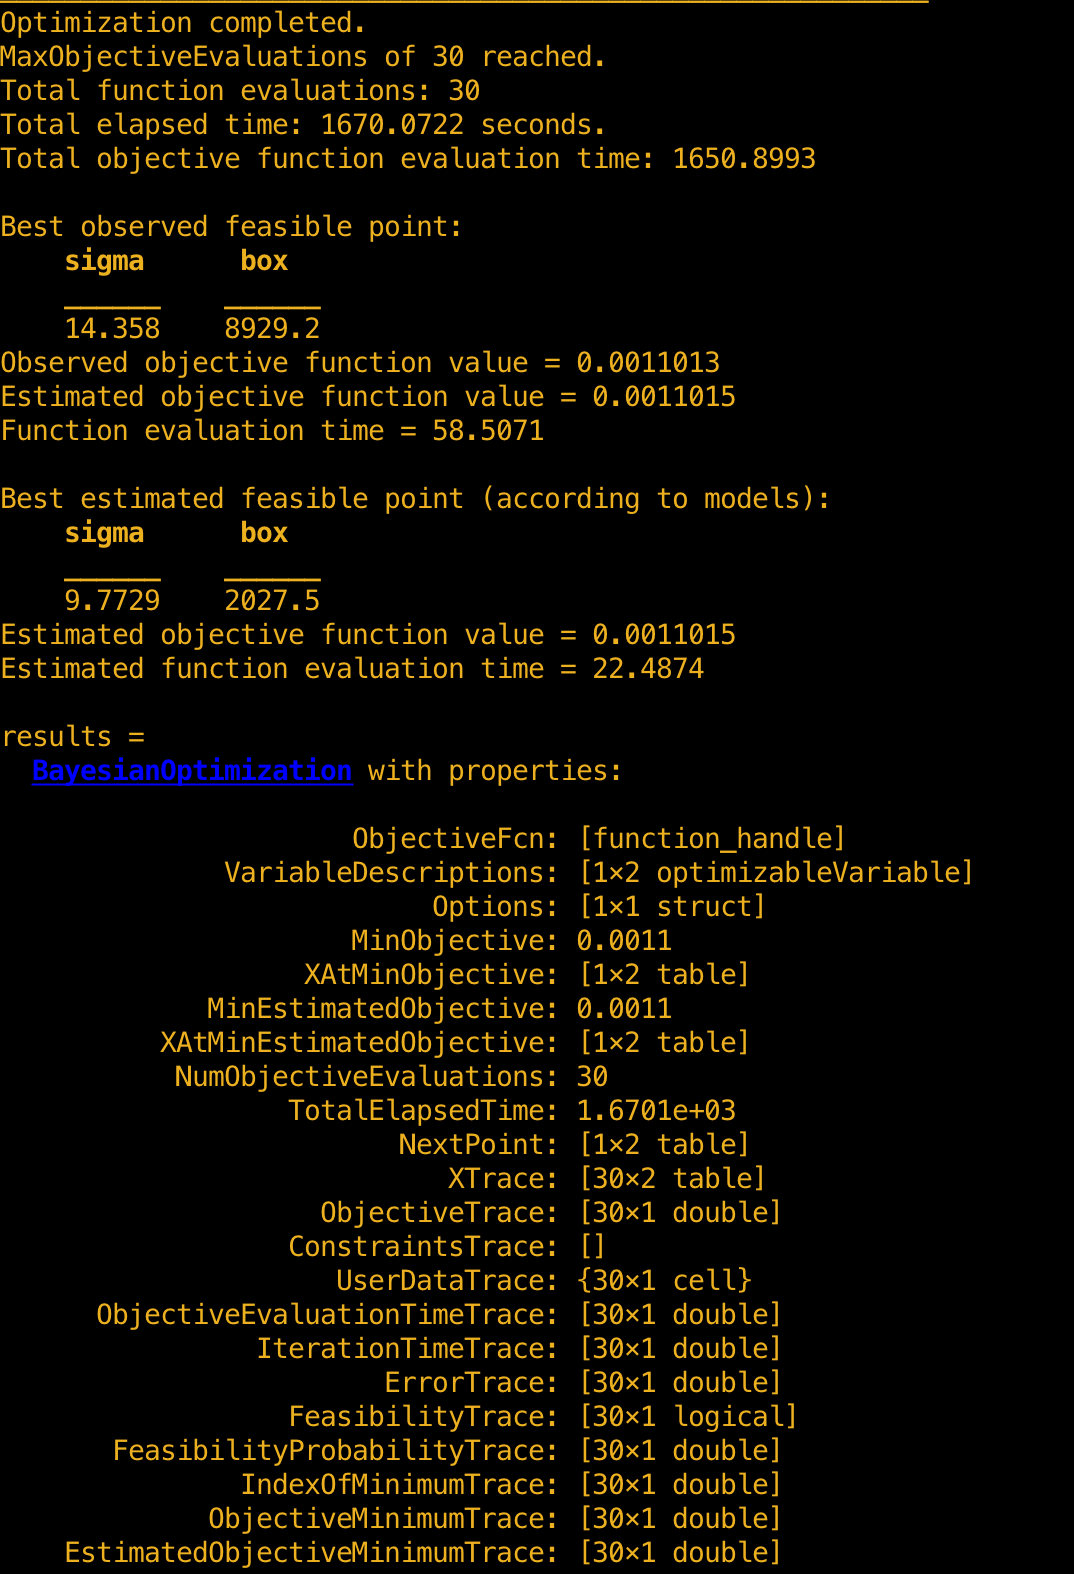
\includegraphics[width=0.93\textwidth]{figures/optimizationResultsStuckFault}    % The printed column width is 8.4 cm.
\caption{Objective function values for different box parameter and sigma values} 
\label{fig:objFuncModel}
\end{center}
\end{figure}

\begin{figure}
\begin{center}
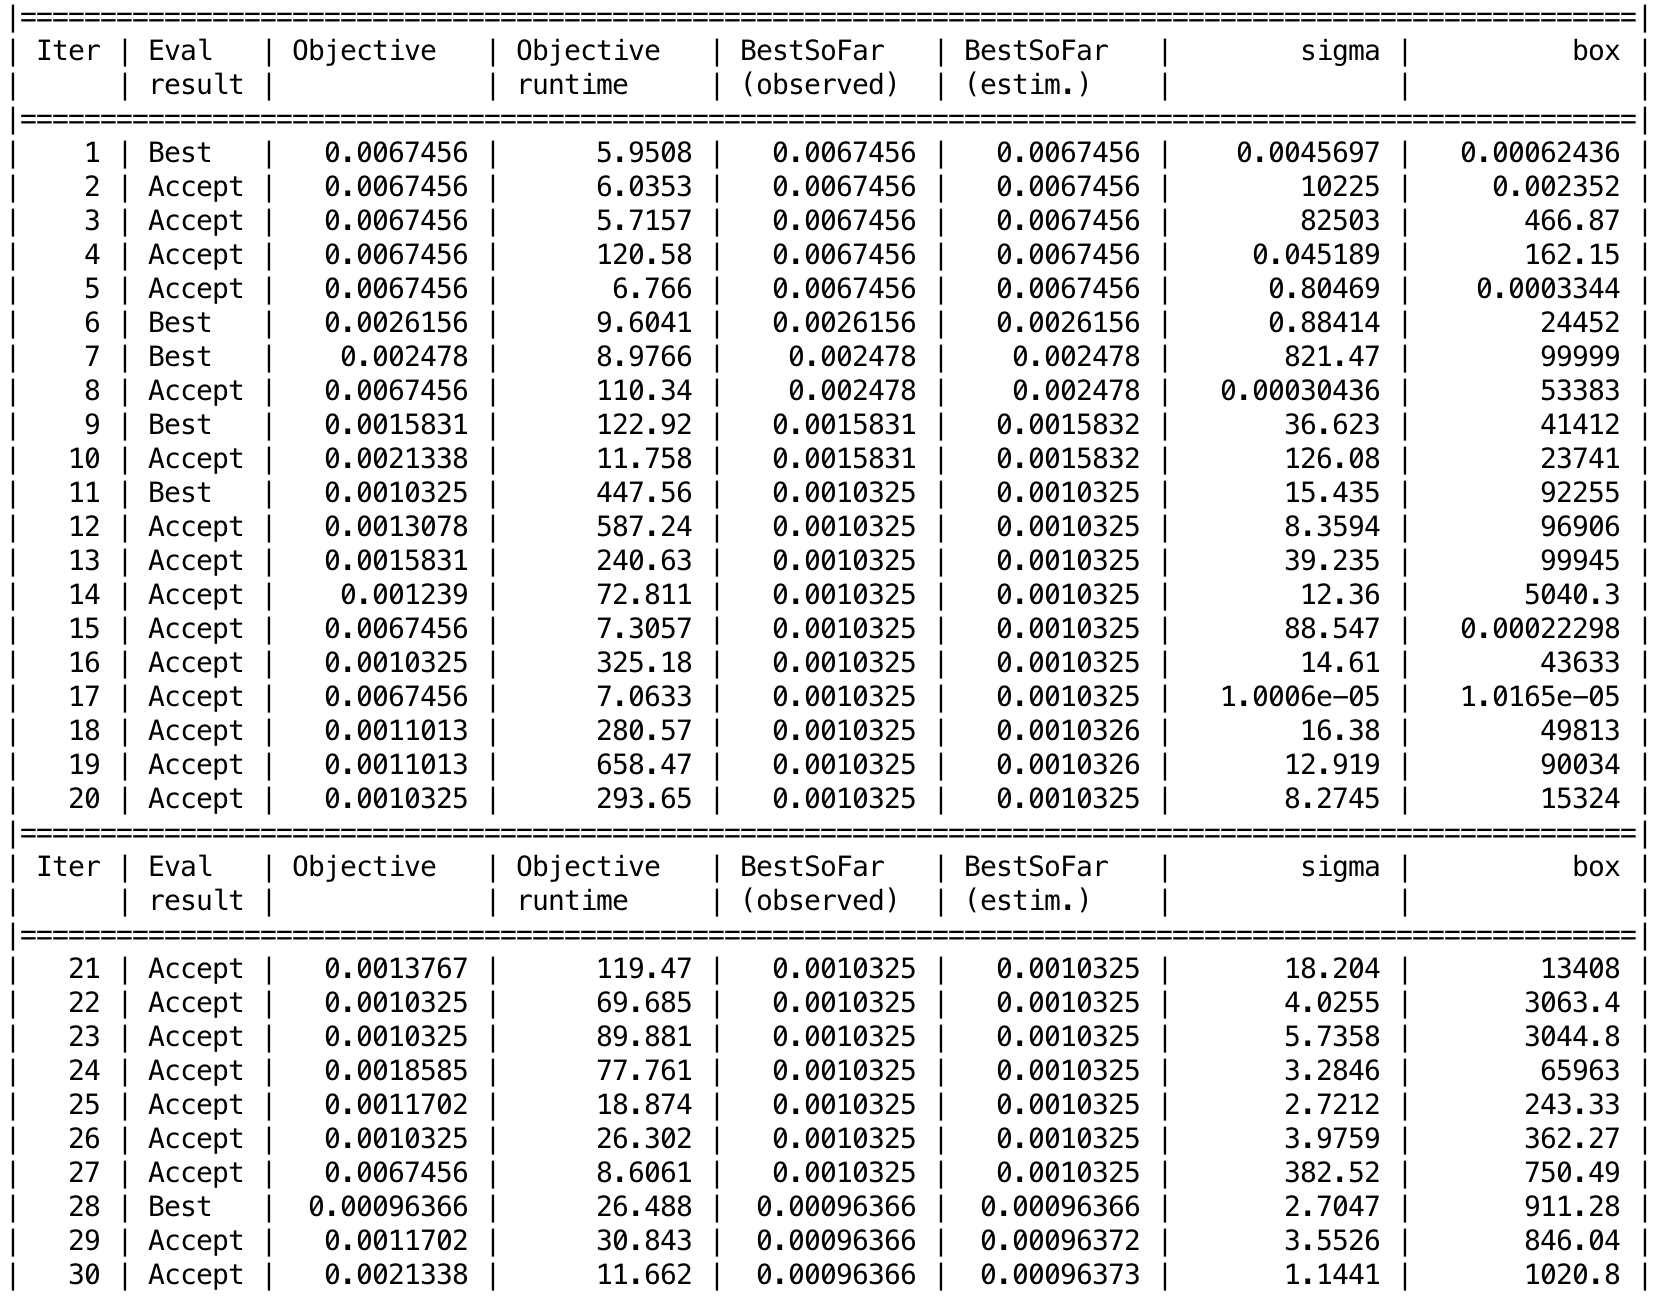
\includegraphics[width=1.13\textwidth]{figures/optimizationSummaryStuckFault}    % The printed column width is 8.4 cm.
\caption{Objective function values for different box parameter and sigma values} 
\label{fig:objFuncModel}
\end{center}
\end{figure}

Two different ways are utilized to tune the classifier, heuristic and Bayesian optimization. In heuristic optimization, the strategy is to try a geometric sequence of the kernel scale (sigma parameter) scaled at the original kernel scale.  Also a geometric sequence of the box constraint parameter, 11 values, from 1e-5 to 1e5 by a factor of 10 have been tried. Increasing box constraint might decrease the number of support vectors, but also might increase training time. Usually, increasing box constraint too much induces overfitting (high variance). 

\begin{figure}
\begin{center}
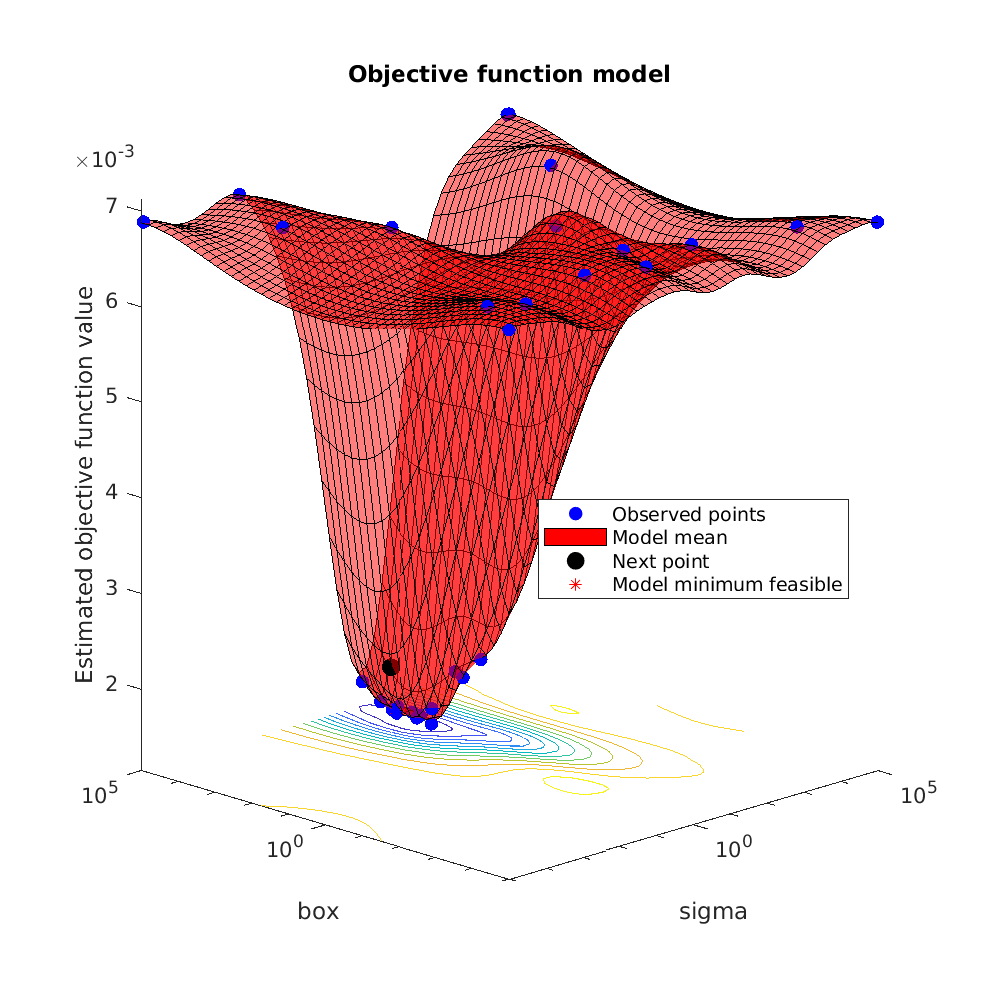
\includegraphics[width=0.7\textwidth]{figures/objFuncModel}    % The printed column width is 8.4 cm.
\caption{Objective function values for different box parameter and sigma values} 
\label{fig:objFuncModel}
\end{center}
\end{figure}


Bayesian optimization tool from Matlab can be used in conjunction with the classification tool to optimize box constraint and the kernel scale. This tool outputs minimum objective value as a function of number of function evaluations (max. number of function evaluations can be changed by passing arguments to the function) as shown in Fig. ~\ref{fig:objectiveFuncEval}. Fig. ~\ref{fig:objFuncModel} shows the objective function values for a variety of box constraint and kernel scale values. The optimized values for box constraint and kernel scale have also been presented in the tables for each classification problem considered.

With a satisfactory result of the training \& tuning is followed by the prediction where the classifier predicts if the new measurement data belongs to the faulty or nominal class. 

\subsubsection{Evaluating the classifier}
\label{evalClassifier}

The performance of the classifier is first quantified by \emph{loss of classification} as indicated with \emph{kFoldLoss} in this work. 
The training data set is  separated to 10 folds. For each fold, the \emph{loss of classification} computed for in-fold observations with a model trained on out-of-fold observations. 
Finally the \emph{loss of classification} is calculated as the \emph{classification error} averaged over all folds.
The idea to split and evaluate the performance of classifiers on different data sets is to avoid overfitting since the fitted classifier would give better results on the data set that it learnt from, but might not generalize well to new data. 
For that reason, both for evaluating the classifiers during tuning phase and finally evaluating the final classifier possessing the tuned parameters, were realized with different data sets.

Another means to evaluate performance of a classifier, available under Matlab Statistics and Machine Learning Toolbox, is via observing the \emph{classification edge}. 
The \emph{edge} is the weighted mean of the \emph{classification margins}. 
Here, the \emph{classification margin} for a binary classifier is defined, for each observation, as the difference between the \emph{classification score} for the \emph{true class} (faulty measurements in the considered problem) and the \emph{classification score} for the \emph{false class} (nominal measurements in the considered problem). 
In this definition, \emph{classification score} is considered as the signed distance from each observation to the decision boundary.

While all these variables would be satisfactory for performance analysis of classifiers, due to the skewed-class nature of the problem, another means of evaluations is necessary.
When the number of instances for different classes in a data set has a big difference, it is named as a skewed-class problem. 
The inherent trickiness to evaluate classifiers for such problems lies on the fact that, predicting only the more frequent class might lead to a misunderstanding that the classifier gives superior performance although it might not be even learning at all. 
For the problem of fault detection of a control surface would serve as a good example to clarify more. 
Since nominal data is not difficult to generate in real flight while it is difficult to fly faulty, the nominal data is much vast compared to the faulty data 

For such problems, in order to define a single metric to evaluate the abilities of classification, \emph{precision} and \emph{recall} should be defined.   
Fig.~\ref{fig:confusionMatrix} shows the confusion matrix which is used to calculate the precision and recall. 
Here, in general, the class indicated by 1 is the skewed class, corresponding to the fault class in this study. 
True positive refers to the number of instances that are predicted faulty and are actually faulty, false positive refers to the number of nominal instances which are miscalculated or predicted as faulty, false negative is the number of instances that are actually faulty but the classifier predicted that they are nominal, and finally the true negative is the number of instances that are predicted as nominal and are actually nominal.
Precision gives a measure on the fraction that was actually faulty of all the measurements that was predicted as faulty. 
Precision can be related to number of false alarms which is cautiously avoided in flight control systems. Precision is defined as 

\begin{figure}
\begin{center}
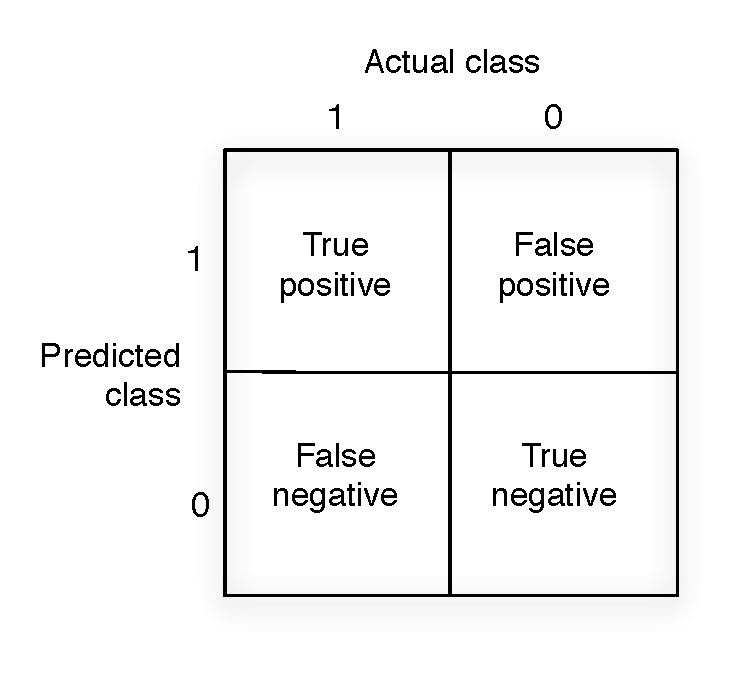
\includegraphics[width=0.5\textwidth]{figures/confusionMatrix}    % The printed column width is 8.4 cm.
\caption{Confusion matrix} 
\label{fig:confusionMatrix}
\end{center}
\end{figure}


\begin{equation}
precision = \frac{true \ positives}{true \ positives + false \ positives}
\end{equation}

Recall refers to the fraction of correctly detected faults of all the situations that was actually faulty. 
Recall can be related to the sensitivity of diagnostic systems. 
Actually an ideal health monitoring system is the one which accomplishes a reasonable balance between the false alarm rate and ability to detect reasonably small faults. 

\begin{equation}
recall = \frac{true \ positives}{true \ positives + false \ negatives}
\end{equation}

Finally as a single metric to evaluate the performance of the classification, F1 score is defined as

\begin{equation}
f1Score = \frac{2 * precision * recall}{precision + recall}
\end{equation}

F1 score, indicated as f1Score in the tables throughout this study is used as the main parameter to evaluate classifiers.

